\documentclass[a6paper, 11pt, parskip=half, DIV=15]{scrartcl}

\usepackage[dvipsnames]{xcolor}
\usepackage{tikz}

\usepackage{ragged2e}
% Minimize unwanted hyphenation
\tolerance=1
\emergencystretch=\maxdimen
\hyphenpenalty=1
\hbadness=10000

\usepackage{fontspec}
\setmainfont{Tex Gyre Schola}
%\setmainfont{Qwigley}

\usepackage{eso-pic}
\usepackage{contour}
\contourlength{0.25mm}
\contournumber{1024}

\definecolor{SunriseBlue}{HTML}{A1A6CF}
\definecolor{brass}{HTML}{FEDB4C}
\definecolor{pine}{HTML}{FCDD68}
\definecolor{redfabric}{HTML}{CB0222}

%\definecolor{SunriseBlue}{HTML}{A9C2E5}
\setkomafont{section}{\setmainfont{Tex Gyre Schola}\LARGE\color{redfabric}\bfseries\scshape}
\setkomafont{subsection}{\setmainfont{Tex Gyre Schola}\Large\color{redfabric}\bfseries}
\setkomafont{subsubsection}{\setmainfont{Tex Gyre Schola}\large\color{redfabric}\bfseries}

% Adjust spacing before and after section headings
\RedeclareSectionCommand[
  runin=false,
  beforeskip=1.0\baselineskip,
  afterskip=-0.0\baselineskip
]{section}

% Adjust spacing before and after subsection headings
\RedeclareSectionCommand[
  runin=false,
  beforeskip=1.0\baselineskip,
  afterskip=-0.0\baselineskip
]{subsection}

% Adjust spacing before and after subsubsection headings
\RedeclareSectionCommand[
  runin=false,
  beforeskip=1.0\baselineskip,
  afterskip=-0.0\baselineskip
]{subsubsection}


\usepackage{enumitem}
\setlist[description]{labelindent=0pt, labelsep=\widthof{ }, leftmargin=\widthof{\textbf{License: }}, font=\setmainfont{Tex Gyre Schola}\bfseries}

\usepackage[hang,flushmargin]{footmisc}
\newcommand\blfootnote[1]{%
  \begingroup
  \renewcommand\thefootnote{}\footnote{#1}%
  \addtocounter{footnote}{-1}%
  \endgroup
}

\renewcommand{\thefootnote}{\fnsymbol{footnote}}
\renewcommand{\footnoterule}{%
  \kern -3pt
  \hrule width \textwidth height 0.5pt
  \kern 2pt
}

\usepackage[hidelinks]{hyperref}
\usepackage[type={CC}, version={4.0}, modifier={by-nc-nd}]{doclicense} % Add text and icons for creative commons license
%\usepackage{array}

\raggedright
\pagestyle{empty}
\begin{document}

\begin{titlepage}
\AddToShipoutPictureBG{
\begin{tikzpicture}[remember picture, overlay]
%	\node () at (current page.center) {\includegraphics[width=\pagewidth, height=\pageheight]{Images/aloft_cover_background.png}};
	\node () at (current page.center) {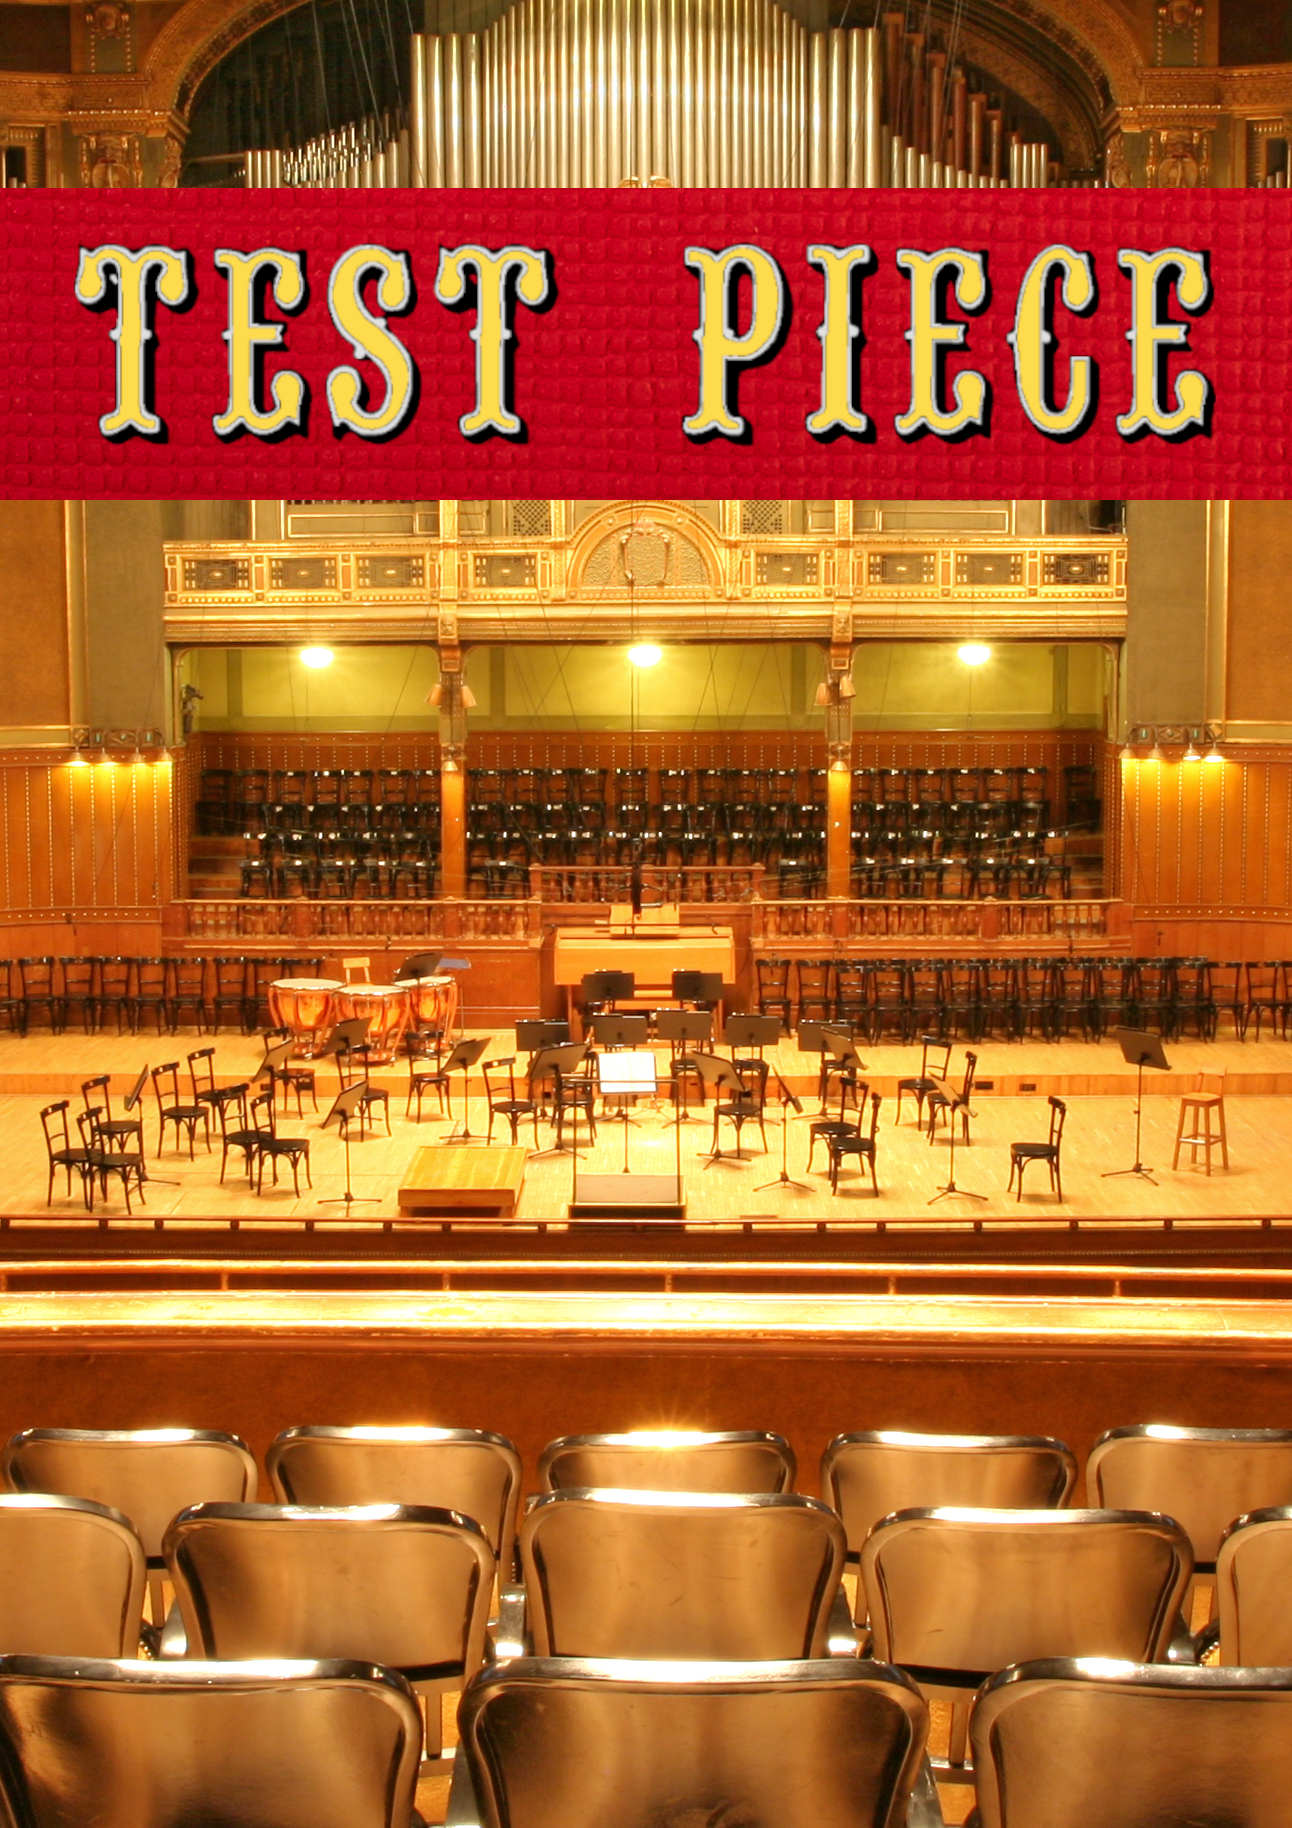
\includegraphics[width=\pagewidth, height=\pageheight]{Images/test_piece_cover.png}};
\end{tikzpicture}
}

\enlargethispage{3.5\baselineskip}
\LARGE
\setmainfont[Scale=1.05]{Playball}
\phantom{test}
\vfill
\begin{center}
\begin{tikzpicture}
\node[draw, black, ultra thick, fill=brass, rounded corners=3mm, text width = 75mm, align=center, text height=2.25ex] at (0,0) {\textcolor{black}{Designed by Michael Purcell}};
\end{tikzpicture}
\end{center}
%\normalsize
%\phantom{a}
\end{titlepage}


\ClearShipoutPicture
\enlargethispage{1.75\baselineskip}
\section*{Overview}
Test Piece is a card-drafting game for two players. It can be played in about thirty minutes and is intended for players who are at least twelve years old.

%During the game, you will launch a flight of hot-air balloons. You will try to ensure that your balloons end up in the best positions in the resulting formation.

%\section*{Components}
%\begin{itemize}[nosep]
%  \item 13 balloon cards
%    \begin{itemize}[nosep]
%      \item 10 regular balloon cards
%      \item 3 special shape balloon cards
%    \end{itemize}
%  \item 13 scoring tokens
%  \item 5 truck cards
%    \begin{itemize}[nosep]
%      \item 4 launch zone truck cards
%      \item 1 safety truck card
%    \end{itemize}
%  \item 5 color cards
%  \item 1 panoramic game board
%\end{itemize}
%
%
%\newpage
%\enlargethispage{1.75\baselineskip}
%\section*{Set Up}
%\begin{enumerate}
%
%  \item Deal one color card at random to each player.
%%  Your color card will determine the color of balloons with which you are \emph{affiliated}.
%  Do not reveal this card to the other players until the end of the game.
%
%%Each regular balloon card is \emph{affiliated} with two of the five possible colors.  The colors that a balloon card is affiliated with are the colors of the envelope of the balloon depicted on that card. Special shape cards are not affiliated with any color.
% 
%  \item Place the launch zone truck cards in a single row below the four leftmost columns of the the game board.% These truck cards comprise the \emph{launch zone}. The leftmost truck card is called the \emph{last truck}. The rightmost truck card in the launch zone is called the \emph{lead truck}.
%
%  \item Place the safety truck card below leftmost launch zone truck card.
%
%%  \item Collect the regular balloon cards and special shape cards that you will use during your game. These cards will comprise the \emph{balloon deck}.
%
%  \item Display the balloon cards in a single row below the launch zone. 
%
%  \item Place the scoring tokens nearby for use when scoring at the end of the game.
%%![Set up for a four-player game.](set_up_diagram.jpg)
%\end{enumerate}
%\begin{center}
%\includegraphics[scale=0.105]{set_up_diagram.jpg}
%\end{center}
%
%\newpage
%\enlargethispage{1.75\baselineskip}
%\section*{Gameplay}
%On your turn, you will perform either one or two actions:
%\begin{enumerate}[nosep]
%  \item If any balloons are flying, move a truck.
%  \item Advance a balloon.
%\end{enumerate}
%
%The game ends when the lead truck moves past the rightmost column of the game board. If this happens on your turn, you should advance a balloon as usual and then proceed to {\setmainfont{Fredoka-Bold} \textcolor{SunriseBlue}{Scoring}}.
%
%\subsection*{Move a Truck}
%If any balloons are flying, then before you advance a balloon you will move a truck. Trucks always move from left to right.
%
%When you move a truck, you will either
%\begin{itemize}[nosep]
%  \item Move a launch zone truck.
%  \item Move the safety truck.
%\end{itemize}
%
%The safety truck must always be between (or even with) the lead truck and the last truck.
%%\begin{itemize}
%%  \item If moving the safety truck would cause it to pass the lead truck, you must move a launch zone truck.
%%  \item If moving a launch zone truck would cause the last truck to pass the safety truck, you must move the safety~truck.
%%\end{itemize}
%
%\subsubsection*{Moving a Launch Zone Truck}
%If the launch zone trucks are in adjacent columns, then you should move the rightmost truck one column to the right.
%
%\begin{center}
%\includegraphics[scale=0.1]{wind_diagram_1.jpg}
%\end{center}
%
%%![Moving a truck when the trucks are in a single group and the safety vehicle is centered on the launch zone.](wind_diagram_1.jpg)
%
%Otherwise, the launch zone trucks will be in two groups which are separated by one empty column. You should move the rightmost truck from the first group one column to the right.
%%It should then be the leftmost truck in the second group.
%
%\begin{center}
%\includegraphics[scale=0.1]{wind_diagram_2.jpg}
%\end{center}
%
%If moving a launch zone truck would cause the last truck to pass the safety truck, then you must move the safety truck.
%
%Any balloon on a launch zone truck should accompany that truck when it is moved.
%
%\newpage
%\enlargethispage{1.75\baselineskip}
%\subsubsection*{Moving the Safety Truck}
%To move the safety truck, you should move it one column to the right.
%
%If moving the safety truck would cause it to pass the lead truck, then you must move a launch zone truck.
%
%\begin{center}
%\includegraphics[scale=0.1]{wind_diagram_3.jpg}
%\end{center}
%
%\subsection*{Advance a Balloon}
%Throughout the game, each balloon will advance through a series of states: packed, unpacked, inflated, and flying at altitudes ranging from one to four. All balloons begin in the packed state.
%
%On your turn, you should advance one balloon of your choice. If you cannot advance any of the balloons, then you should skip this step.
%
%\newpage
%To advance a balloon, you should move it from its current state to the next.
%\begin{description}[leftmargin=0pt]
%  \item[Unpack:] To advance a balloon from the packed state to the unpacked state, place it horizontally on a launch zone truck.
%  \begin{itemize}
%    \item You may not place a balloon on a truck that already has a balloon on it.
%  \end{itemize}
%  \item[Inflate:] To advance a balloon from the unpacked state to the inflated state, turn it so that it is placed vertically on its truck.
%  \item[Launch:] To advance a balloon from the inflated state to the flying state, move it to the bottom row of the game board above its truck. It will then be flying at an altitude of one.
%  \item[Ascend:] To advance a balloon that is flying, move it up one row. It will then be flying at an altitude one more than before.
%  \begin{itemize}
%    \item Balloons that are flying may never be orthogonally adjacent to one another.% balloon which is flying.
%    \item The maximum altitude at which balloons can fly is four.
%  \end{itemize}
%\end{description}
%
%\newpage
%\enlargethispage{1.75\baselineskip}
%\subsection*{Scoring}
%%Each balloon scores a number of points that is determined by its position within the formation. In general, balloons that are flying at higher altitudes score more points than those that are flying at lower alititudes.  If balloons are flying at the same altitude, then the balloons that are closer to the front (right-hand side) of the formation score more points than the balloons that are closer to the back (left-hand side) of the formation. 
%
%Use the scoring tokens to indicate the number of points scored by each balloon.
%\begin{enumerate}
%  \item Place the scoring token numbered ``1'' on the leftmost balloon in the bottom row of the formation.
%  \item Scanning from left to right and bottom to top, place scoring tokens on the other balloons in the formation, placing the token with lowest remaining number on each balloon as you encounter it.
%%  \item Proceed to the next highest row of the formation. Continue in this fashion, scanning from left to right and bottom to top, until each balloon that is flying has been assigned a scoring token.
%\end{enumerate}
%
%%Notice that the leftmost balloon in the bottom row of the formation always scores one point while the rightmost balloon in the top row of the formation scores one point for every balloon that is flying at the end of the game. See the figure below for a more complete example.
%
%Your score is the sum of the scores for all of the balloons with which you are affiliated (i.e. that match your color card). The player with the highest score wins the game.
%
%\begin{center}
%\includegraphics[scale=0.115]{scoring_diagram.jpg}
%\end{center}
%
%\newpage
%\enlargethispage{1.75\baselineskip}
%\section*{Solo Mode}
%Aloft can also be played as a one-player game.
%\blfootnote{\textbf{Contact}: \href{mailto:aloft.board.game@gmail.com}{aloft.board.game@gmail.com}}
%\blfootnote{\textbf{License}: \raggedright\doclicenseLongText}
%This is similar to the multi-player version, differing in the following ways:
%\begin{itemize}
%  \item You will not use the color cards or the scoring tokens. You will only use two of the special shape balloon cards.
%  \item You will shuffle the balloon cards before dealing them out in a single row below the game board. If you choose to unpack a balloon on a given turn, you must unpack the first (leftmost) remaining balloon.
%  \item Balloons that are flying and that share a color may never be diagonally adjacent to one another.
%  \item Your score is equal to the number of adjacent columns required to contain the formation plus a three point penalty for every balloon which you failed to launch.
%\end{itemize}
% \newpage
% \AddToShipoutPictureBG{
%\begin{tikzpicture}[remember picture, overlay]
%%	\node () at (current page.center) {\includegraphics[width=\pagewidth, height=\pageheight]{Images/aloft_cover_background.png}};
%	\node () at (current page.center) {\includegraphics[width=\pagewidth, height=\pageheight]{Images/aloft_back_cover_background.png}};
%\end{tikzpicture}
%}
%\phantom{Aloft}
%\vfill
%\begin{center}
%{\setmainfont{Fredoka-Bold}\huge\textcolor{white}{The Balloonist's Prayer}\\[2ex]}
%\textcolor{white}{May the winds welcome you with softness.\\[2ex]
%May the sun bless you with its warm hands.\\[2ex]
%May you fly so high and so well that God\\[2ex]
%joins you in laughter and sets you gently\\[2ex]
%back into the loving arms of Mother Earth.}
%\end{center}
%%\vfill
%\phantom{Aloft}
%
%\phantom{Aloft}
\end{document}